% ============================================================
% TCCML @ NeurIPS 2026 (Papers track): HARD 4-page main-body limit,
% references excluded from the count (per the official CFP PDF the user
% attached). Round 7 (Aug 29): rebuilt for the real page budget --
% single-column, 5.5in x 9in text block, dense prose, figures shrunk and
% combined two-per-row to cut vertical space, appendix (Q-sweep detail,
% phase-out scenario, training/convergence methodology, what was tried
% and rejected) kept AFTER the bibliography since the CFP explicitly
% allows supplementary appendices at reviewer discretion and they do not
% count against the 4-page limit. Every number below is unchanged from
% the verified round-6 draft -- only presentation/formatting changed
% this round, nothing was re-run.
%
% NOTE ON AUTHORSHIP: names/affiliations filled in for internal Overleaf
% collaboration. Restore to "Anonymous Author(s)" before actual
% submission -- TCCML review is double-blind.
% ============================================================

\documentclass{article}
% The style file loads natbib itself; ask for numeric, sorted-and-compressed
% citations before it does (matches the citation format used across our
% other TCCML submission).
\PassOptionsToPackage{numbers,sort&compress}{natbib}
\usepackage[final]{neurips_2026}

\usepackage[utf8]{inputenc}
\usepackage[T1]{fontenc}
\usepackage{hyperref}
\usepackage{url}
\usepackage{booktabs}
\usepackage{amsfonts}
\usepackage{amsmath}
\usepackage{nicefrac}
\usepackage{microtype}
\usepackage{graphicx}
\usepackage{xcolor}
\usepackage{tikz}
\usepackage{float}
\usetikzlibrary{arrows.meta,positioning}

\newcommand{\todo}[1]{\textcolor{red}{\textbf{[TODO: #1]}}}

% Tightened float/vertical spacing to reclaim room for the new Sec.~1
% paragraph and Sec.~5 clause without touching figure sizes/fonts or
% restructuring anything -- keeps the main body at 4 pages.
\setlength{\textfloatsep}{5pt plus 2pt minus 2pt}
\setlength{\intextsep}{4pt plus 2pt minus 2pt}
\setlength{\floatsep}{4pt plus 2pt minus 2pt}
\setlength{\abovecaptionskip}{3pt}
\setlength{\belowcaptionskip}{1pt}
\setlength{\abovedisplayskip}{5pt plus 2pt minus 2pt}
\setlength{\belowdisplayskip}{5pt plus 2pt minus 2pt}
\setlength{\abovedisplayshortskip}{3pt plus 2pt minus 2pt}
\setlength{\belowdisplayshortskip}{3pt plus 2pt minus 2pt}
\setlength{\parskip}{3.4pt}

\title{Methane First: A Physically-Consistent Framework for Sequencing
Climate Cleanup Investment in the AI Data Center Buildout}

\author{
  Anonymous Author(s) \\
  Affiliation \\
  Address \\
  \texttt{email}
}

\begin{document}
\maketitle

\begin{abstract}
Data center development is caught between two forces: hyperscale demand
driving trillions in capital spending
\cite{bloombergnef2025aipowergrid,ucs2026datacenterpowerplay}, and
growing local resistance over grid strain, water, land, and the
greenhouse gases these sites emit
\cite{gallup2026opposedatacenters,umich2025datacentersimpact}.
Developers rush to build at top speed and treat those costs as an
afterthought, but speed without foresight is a liability, starting with
the fuel itself. Off-grid natural gas is becoming this buildout's
\emph{transient} bridge fuel, and current reporting folds its methane
and CO$_2$ emissions into one
number using a hundred-year comparison built for carbon dioxide alone
\cite{eip2026powerbehindai}. That hides something important: methane
warms hard and fast, then fades away within a couple of decades, while
CO$_2$'s warming barely fades at all, so the time window you use to
judge a decarbonization investment changes which one looks smart. We
study this on a real fleet of 69 U.S. data centers running their own
on-site gas turbines, first treating leak repair (LDAR) as a one-time
purchase on that fixed fleet, then, more realistically, as a cost paid
every year on a fleet that grows to 350 data centers by 2035. We train
a reinforcement learning policy to split a fixed budget between LDAR
and carbon capture (CCS), and the winning strategy flips entirely with
the climate metric: LDAR first under the 20-year lens that matches
these plants' own short lifespan, CCS first under the 100-year
convention nearly every report defaults to. No model that treats leak
repair as a one-time purchase can see this crossover, yet it is a real
choice already being made by default on a fleet set to scale five-fold
by 2035. Get it wrong, and the industry locks in the wrong technology
for plants that were never meant to last. Get it right, and AI's race
to power itself becomes proof that the world's fastest-growing
industry can also be its fastest to clean up after itself.
\end{abstract}

\section{Introduction}
\label{sec:intro}

AI is driving one of the largest waves of infrastructure construction in
history, and in that race, speed matters more than almost anything else.
Waiting years for a new grid connection is often not an option, so many
new data centers are instead being built with their own on-site natural
gas power plants. The industry treats this as a temporary fix: a stopgap
that will be phased out as nuclear power and other clean, reliable
sources of electricity come online over the next decade or two
\cite{eip2026powerbehindai}.

A temporary fix still has real costs today. Burning that gas releases
carbon dioxide, which lingers in the atmosphere for roughly a century,
and leaks methane, both upstream and directly from the plants
themselves; in this paper, LDAR (leak detection and repair) means
cleanup for both leak pathways. Most reporting converts both gases into
one number, called CO$_2$-equivalent, using carbon dioxide's
hundred-year timescale as the yardstick for both. That hides something
important: methane's warming effect is strongest in its first couple of
decades and mostly fades after that, while carbon dioxide's warming
barely fades at all, and since these plants are themselves meant to be
short-lived, the time window used to judge them changes which cleanup
investment looks smart.

This paper asks a simple question: given a fixed annual cleanup budget,
how should it be split between LDAR and carbon capture (CCS), and does
the answer change with the metric used to judge it? We build a
two-phase model (Sec.~\ref{sec:methods}) on a real set of gas-powered
data centers and train a reinforcement learning policy to answer it,
using a climate layer adapted from Cui et al.'s aviation-FAIR framework
\cite{cui2024aviationfair,millar2017fair,smith2018fair,joos2013carbon}
and the same 20-year/100-year dual-horizon lens as Sartzetakis et al.\
\cite{sartzetakis2025temporaltradeoffs}, echoing the ``timing versus
allocation'' trade-off Bauer et al.\ describe for climate policy
generally \cite{bauer2024timing}, applied here within one asset class
across two cleanup technologies. To our knowledge, this is the first
framework to expose data center climate-cleanup spending to a
metric-aware, year-by-year policy instead of one fixed rule, pointing
toward adaptive, AI-driven policymaking as one way to address the AI
boom's own negative externalities.

\section{Data and Methods}
\label{sec:methods}

\textbf{Fleet and baseline.} We start from a real, EIP-reported inventory
of 74 proposed, permitted, or operating U.S. gas-turbine data center
facilities \cite{eip2026powerbehindai}, keeping the \textbf{69} with
usable capacity and permit data. For each facility we compute gas
throughput, upstream leaked methane from a basin-specific leak rate
(Permian 9.4\%, Appalachian 0.52\%, 2.3\% elsewhere on average
\cite{chen2022permian,ami2025appalachian,alvarez2018methane}), and
CO$_2$ from its EIP-reported total; the fleet averages 2{,}048 MW and
about 108,000 t/yr of upstream CH$_4$. Our GWP20 and GWP100 weights
(92.1 and 30.9) come from this paper's own FAIR-adapted pulse response
and set the reward throughout. \textbf{LDAR}, as defined in
Sec.~\ref{sec:intro}, covers both upstream repair and engine-level
methane slip: AP-42 industry-average factors put reciprocating engines,
increasingly used on new sites, at roughly $145\times$ more methane per
unit of fuel than turbines, and equipment-specification estimates for
one already-permitted site put its slip alone on the same order as a
single average facility's upstream total in our fleet
\cite{epa1996ap42,wvdep2026pointpleasant}. LDAR costs \$6--17/tCO$_2$e
for most addressable reduction, steepening past $\sim$70\% deployment
\cite{icf2014methane,iea2025methanetracker,aldy2025methaneabatement};
\textbf{CCS} costs \$56--71/tCO$_2$e, roughly flat across 90--97\%
capture \cite{rubinzhai2012ccs,netl2023ngcc}.

\textbf{Phase A: fixed fleet, LDAR as a one-time purchase.} Phase A holds
the fleet at 69 facilities and treats LDAR as a one-time purchase, a
capital expense: a deployment fraction only ratchets upward toward a
\textbf{95\% ceiling}, and once bought, abatement is permanent (CCS the
same way, with a 90\% ceiling). Phase A has no floor $Q$; that only
matters once LDAR is a recurring flow that can drift back toward doing
nothing, in Phase B. We compare five candidate policies here, including
one trained with REINFORCE~\cite{williams1992reinforce}.

\textbf{Phase B: growing fleet, LDAR as a yearly expense.} In practice,
leaks reappear, so LDAR is really something you keep paying for. Phase B
models that directly: the fleet $n(t)$ follows a real, dated schedule
(dcmap.us, Aug.\ 2026), growing 69 to 350 facilities by 2035 and held
flat after that (Fig.~\ref{fig:nt}). LDAR is now an \textbf{operating
expense}: each year's realized leak rate is a memoryless flow,
\begin{equation}
  \ell(t) \;=\; P \;-\; (P - Q)\,\phi(t), \qquad \phi(t) \in [0,1],
  \label{eq:leakrate}
\end{equation}
where $\ell(t)$ is year $t$'s realized leak rate, $P=3.11\%$ is the
real, throughput-weighted do-nothing rate, $Q$ is the best sustainable
floor reachable under maximum annual spend, and $\phi(t)\in[0,1]$ is
that year's LDAR spend divided by what holding the floor $Q$ costs for
one year. Spending nothing gives $\ell(t)=P$; spending the full amount
gives $\ell(t)=Q$; skipping a year drifts $\ell(t)$ back toward $P$
immediately, with no credit for past investment. We report three
floors, $Q\in\{0\%, 1.5\%, 3.1\%\}$: fully sealed, our recommended
headline floor, and a floor barely below $P$ where spending does almost
nothing (full sweep in Appendix~\ref{sec:app-qsweep}).

\begin{figure}[h]
  \centering
  \begin{minipage}[c]{0.36\linewidth}
    \centering
    \includegraphics[width=\linewidth]{figures/nt_mw_dual_axis.png}
  \end{minipage}%
  \hfill
  \begin{minipage}[c]{0.60\linewidth}
    \centering
    \resizebox{\linewidth}{!}{%
    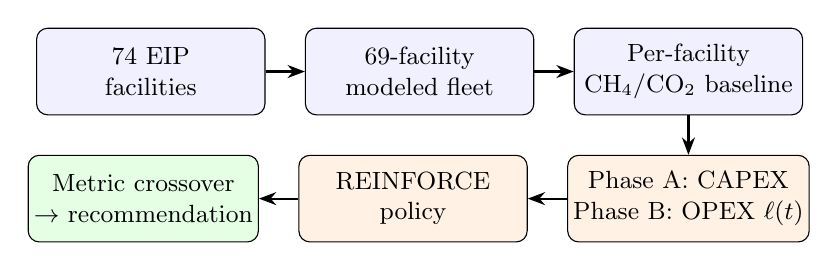
\begin{tikzpicture}[
      node distance=5mm and 5mm,
      box/.style={draw, rounded corners, fill=blue!6, align=center, minimum height=11mm,
                  minimum width=29mm, font=\small, inner sep=2pt},
      ab/.style={box, fill=orange!10},
      outbox/.style={draw, rounded corners, fill=green!10, align=center, minimum height=11mm,
                     minimum width=29mm, font=\small, inner sep=2pt},
      arr/.style={-{Stealth[length=2.2mm]}, thick}
    ]
      \node[box] (inv) {74 EIP\\facilities};
      \node[box, right=of inv] (fleet) {69-facility\\modeled fleet};
      \node[box, right=of fleet] (base) {Per-facility\\CH$_4$/CO$_2$ baseline};
      \node[ab, below=of base] (ab) {Phase A: CAPEX\\Phase B: OPEX $\ell(t)$};
      \node[ab, left=of ab] (rl) {REINFORCE\\policy};
      \node[outbox, left=of rl] (out) {Metric crossover\\$\to$ recommendation};
      \draw[arr] (inv) -- (fleet);
      \draw[arr] (fleet) -- (base);
      \draw[arr] (base) -- (ab);
      \draw[arr] (ab) -- (rl);
      \draw[arr] (rl) -- (out);
    \end{tikzpicture}}
  \end{minipage}
  \caption{\emph{Left:} the fleet-growth input $n(t)$ driving Phase B,
  69$\to$350 facilities by 2035 (dcmap.us schedule), held flat thereafter.
  \emph{Right:} pipeline from the raw facility inventory to the policy
  recommendation.}
  \label{fig:nt}
\end{figure}

\section{Results}
\label{sec:results}

\textbf{Phase A: LDAR first, and the metric does not matter here.} In
this simpler model, LDAR is bought once and kept forever, a baseline for
what happens when the metric choice (GWP20 vs.\ GWP100) has nothing to
bite into, before Phase B, where it does. RL, the greedy rule, and LDAR
first all converge to the \emph{same} allocation curve under both
metrics (Fig.~\ref{fig:phaseA}, top), and LDAR first beats every fixed
policy in cumulative avoided CO$_2$e under both (Fig.~\ref{fig:phaseA},
bottom): the metric changes reward magnitude, not which policy wins.
RL's own training curve (Appendix, Fig.~\ref{fig:phaseA-train-app})
confirms there is no real sequential decision here, since one policy
already wins under both.

\begin{figure}[h]
  \centering
  \includegraphics[width=0.92\linewidth]{figures/phaseA_allocation_ratio.png}\\[0pt]
  \includegraphics[width=0.92\linewidth]{figures/phaseA_cumulative.png}
  \caption{Phase A, GWP20 (left panel of each) vs.\ GWP100 (right panel
  of each). \emph{Top:} LDAR's share of the yearly budget (CCS share is 1
  minus this); panels are pixel-identical here. \emph{Bottom:} cumulative
  avoided CO$_2$e, end values labeled. RL/LDAR-first outruns CCS-first
  ($\sim$4$\times$ GWP20, $\sim$1.9$\times$ GWP100); its edge over 50/50
  is modest here (+2.5\%/+1.5\%) -- Phase B is where it grows large
  (Fig.~\ref{fig:phaseB}).}
  \label{fig:phaseA}
\end{figure}

\textbf{Phase B: once LDAR is a recurring cost, the two metrics disagree.}
Now we make LDAR behave like it really does: something you pay for every
year, the way Sec.~\ref{sec:methods} sets up Phase B. Fig.~\ref{fig:phaseB}
(top) shows what the trained policy does under each metric: under GWP20
it shifts toward more LDAR over time (67\% to 73\% of the budget); under
GWP100 it shifts the other way (49\% down to 37\%, toward more CCS).
\textbf{This is the paper's central result:} once LDAR is modeled
honestly, as a bill paid every year rather than a purchase made once,
the two metrics genuinely disagree, something Phase A never shows. Why:
CCS buys a permanent captured fraction that pays off longer the earlier
it is bought; LDAR only buys that one year's leak rate, with nothing
carried forward. A 20-year window rewards the cheaper, immediate LDAR
fix; a 100-year window rewards CCS's permanence instead. In cumulative
avoided CO$_2$e (Fig.~\ref{fig:phaseB}, bottom), the trained policy
beats a fixed 50/50 split by \textbf{6.5\%} under GWP20 and
\textbf{4.3\%} under GWP100, over 2025 to 2100 undiscounted (93.8 vs.\
88.0 Gt; 57.5 vs.\ 55.1 Gt), an advantage that grows to $+71.8\%$
(GWP20) as the floor $Q$ approaches $P$, where a naive 50/50 split
wastes half its budget chasing a floor already nearly met. A constant-split
sweep confirms the same lean, LDAR-heavy under GWP20, CCS-heavy under
GWP100, at $Q=0\%$ and $1.5\%$ (Appendix~\ref{sec:app-qsweep}).
Fig.~\ref{fig:phaseB-train} confirms the policy learns this: best-so-far
reward levels off well before the 3{,}000-episode budget and clears
fixed 50/50 under both metrics.

\begin{figure}[!h]
  \centering
  \includegraphics[width=0.80\linewidth]{figures/phaseB_dual_allocation_ratio.png}\\[0pt]
  \includegraphics[width=0.80\linewidth]{figures/phaseB_dual_cumulative.png}
  \caption{Phase B at $Q=1.5\%$, GWP20 vs.\ GWP100. \emph{Top:} LDAR's
  share of the yearly budget (CCS share is 1 minus this): GWP20 drifts
  toward more LDAR, GWP100 toward more CCS, the crossover Phase A never
  shows. \emph{Bottom:} cumulative avoided CO$_2$e.}
  \label{fig:phaseB}
\end{figure}

\begin{figure}[h]
  \centering
  \begin{minipage}[c]{0.55\linewidth}
    \centering
    \includegraphics[width=\linewidth]{figures/phaseB_training_curve_gwp20.png}
  \end{minipage}%
  \hfill
  \begin{minipage}[c]{0.40\linewidth}
    \centering
    \small
    \begin{tabular}{lr}
      \toprule
      Metric & RL adv.\ \\
      \midrule
      GWP20  & $+6.5\%$ \\
      GWP100 & $+4.3\%$ \\
      \bottomrule
    \end{tabular}
    \vspace{3pt}

    \raggedright
    \footnotesize vs.\ Fixed 50/50, undiscounted, 2025--2100, $Q=1.5\%$.
  \end{minipage}
  \caption{Phase B training curve, GWP20, $Q=1.5\%$: best-so-far reward
  plateaus early and clears Fixed 50/50. Table: RL advantage, both metrics.}
  \label{fig:phaseB-train}
\end{figure}

\textbf{Why the horizon matters: a check at 2050.} Most net-zero
commitments target 2050, not 2100. RL is already \textbf{27.9\% ahead}
of fixed 50/50 under GWP20 at that horizon (Table~\ref{tab:2050}), but
still \textbf{1.8\% behind} under GWP100, not pulling ahead until 2063.
Since these facilities are themselves short-lived, GWP20 is the more
decision-relevant metric here.

\begin{table}[H]
  \caption{RL vs.\ fixed 50/50, $Q=1.5\%$: avoided CO$_2$e (Gt, undisc.), 2050 vs.\ 2100.}
  \label{tab:2050}
  \centering
  \small
  \begin{tabular}{lrrr}
    \toprule
    Metric & Year & RL / Fixed 50/50 (Gt) & RL adv. \\
    \midrule
    GWP20  & 2050 & 26.16 / 20.46 & $+27.9\%$ \\
    GWP20  & 2100 & 93.76 / 88.00 & $+6.5\%$ \\
    GWP100 & 2050 & 9.72 / 9.91   & $-1.8\%$ \\
    GWP100 & 2100 & 57.46 / 55.10 & $+4.3\%$ \\
    \bottomrule
  \end{tabular}
\end{table}

\textbf{Robustness.} A sweep of all 11 constant LDAR/CCS splits confirms
the trained policy lands within a few percent of the true ceiling in
every phase, floor, and metric tested (Appendix~\ref{sec:app-qsweep});
retiring the gas fleet linearly to zero by 2045 still leaves RL beating
fixed 50/50 by 41.9\% (GWP20) and 12.7\% (GWP100) while the fleet exists
(Appendix~\ref{sec:app-phaseout}).

\section{Discussion \& Conclusion}

What matters is not that a learned policy beats a simple heuristic, but
that the right investment changes once leak repair is modeled as it
really works: a bill due every year, not a one-time purchase. Under the
standard 100-year convention, CCS looks right first; under the more
honest 20-year lens, for a fleet of data centers the industry itself
calls transient, LDAR does instead. A regulator picks a side of this
split by choosing a reporting metric on a fleet set to scale $5\times$
in a decade (Sec.~\ref{sec:methods}), often without realizing it:
GWP100 by habit means spending the early years doing the opposite of
what the 20-year lens recommends, while these facilities still exist
(Table~\ref{tab:2050}), a wrong-direction default for a temporary asset
class. And
that choice is being made right now: this buildout is still early
enough to get it right, and too large to get it wrong. Separating
methane from carbon dioxide, instead of averaging them away into one
convenient number, is not a footnote to this story, it is the story. It
is the difference between an industry that cleans up as it grows and
one that spends the next decade quietly correcting itself. Measuring
the climate cost of AI honestly, at the speed AI itself is moving, is
one of the more consequential and still wide-open problems in climate
work today.

\bibliographystyle{plainnat}
\bibliography{references}

\appendix
\section{Appendix: modeling process, robustness checks, and supplementary results}
\label{sec:appendix}
{\small
Per the workshop CFP, appendices do not count against the 4-page limit
and are read at reviewer discretion; this one documents what was
actually tried, not just the plots that made the main text.

\subsection{RL training procedure and convergence verification}
\label{sec:app-rl}

Both phases use the identical REINFORCE policy-gradient algorithm
\cite{williams1992reinforce}: a two-layer network with a $\tanh$ hidden
layer maps the state (year index, allocation share, and, in Phase B, the
growth factor) to the mean of a bounded Gaussian over next year's LDAR
budget share, $a\sim\mathcal{N}(\mu,0.15)$, clipped to $[0,1]$; CCS gets
$1-a$. Each episode replays 2025--2100 once; the update is a standard
reward-to-go policy gradient with a scalar batch-mean baseline (lr
$0.02$), no value network, no entropy bonus, no reward shaping beyond
the $2\%$ annual discount already in the reward. The same hyperparameters
were reused, unmodified, across all eight (phase, $Q$, metric)
configurations in this paper, itself a robustness signal that no
reported crossover is an artifact of per-configuration tuning.

We trained for 3{,}000 episodes/configuration. Rather than trust a reward
curve's shape alone, we independently computed a \textbf{fixed-share
sweep}: rerun the environment at 11 constant shares $\{0.0,\dots,1.0\}$
(no learning) and take the max, a model-independent check on which
constant policy is actually best (Table~\ref{tab:qsweep-adv}'s ``best
fixed share'' column), verified at generation time against an assertion
that the sweep's argmax matches the fixed-policy trajectory data (this
caught a mismatched-$Q$ bug on an early Phase B run). The training-curve
figures themselves (Figs.~\ref{fig:phaseB-train},
\ref{fig:phaseA-train-app}) plot RL only against Fixed 50/50, the
benchmark this paper's headline numbers are stated against, rather than
against that extreme swept corner, a policy-gradient method samples its
actions from a distribution with a fixed exploration variance
(Sec.~\ref{sec:app-rl}), so it can get close to but rarely lands exactly
on a $100\%$-to-one-technology corner solution even once it has correctly
identified that corner as best; the (small) gap to that corner is a
property of the training procedure, not evidence RL failed to learn the
right answer, and it does not affect any advantage number reported in
this paper, all of which are against Fixed 50/50. Fig.~\ref{fig:phaseA-train-app}
shows Phase A's own training curve: RL, greedy, and LDAR-first converge
to the same curve under both metrics from very early on, confirming Phase
A's permanent-CAPEX formulation has a single dominant strategy and no
metric-dependent trade-off for RL to discover, which is why it lives
here, not in the main text; the genuinely novel training dynamic is Phase
B's (Fig.~\ref{fig:phaseB-train}).

\begin{figure}[h]
  \centering
  \includegraphics[width=0.92\linewidth]{figures/phaseA_training_curve.png}
  \caption{Phase A training curve vs.\ fixed baselines: RL, greedy, and
  LDAR-first converge to the same curve under both metrics.}
  \label{fig:phaseA-train-app}
\end{figure}

We also directly tested whether Phase B's OPEX mechanic does real work,
versus being Phase A with extra parameters: freezing Phase B's growth
factor at 1 reproduces Phase A's raw emissions baseline exactly (max abs.
diff.\ $0.000000$ tons, both gases), but the \emph{policy} comparison
does not collapse, Phase A's LDAR share persists forever once bought,
while Phase B's leak rate reverts toward $P$ every unfunded year
(Eq.~\ref{eq:leakrate} has no memory), producing a $+14.85\%$
RL-vs-fixed advantage on the frozen-growth Phase B fleet where true
Phase A shows a materially different number on the identical fleet --
evidence the two phases are structurally different models, not the same
model at different settings.

\subsection{Full $Q$-sweep}
\label{sec:app-qsweep}

$Q$ has no literature value, so we swept $Q=0\%$ (perfect repair),
$1.5\%$ (headline, midpoint), and $3.1\%\approx P$ (floor barely better
than nothing); all runs use Sec.~\ref{sec:methods}'s equations, only $Q$
changes, propagating through $\phi_{\text{target}}=1-Q/P$ and the dollar
cost to reach the floor.

\begin{table}[h]
  \caption{Cost to reach the LDAR floor vs.\ $Q$; both fall as $Q\to
  P=3.11\%$.}
  \label{tab:qsweep-cost}
  \centering
  \small
  \begin{tabular}{lrrr}
    \toprule
    $Q$ & $\phi_{\text{target}}$ & One-time cost & Annual OPEX \\
    \midrule
    $0\%$   & $1.0000$ & \$2{,}218.2M & \$221.8M/yr \\
    $1.5\%$ & $0.5177$ & \$793.4M     & \$79.3M/yr \\
    $3.1\%\ (\approx P)$ & $0.0033$ & \$4.4M & \$0.4M/yr \\
    \bottomrule
  \end{tabular}
\end{table}

\begin{table}[h]
  \caption{RL vs.\ fixed 50/50, all six $(Q,$ metric$)$ combos, 2025--2100
  undiscounted. The metric crossover (best share $=1.0$ under GWP20 vs.\
  $=0.0$ under GWP100) holds at $Q=0\%$ and $Q=1.5\%$; at $Q=3.1\%$ both
  metrics prefer CCS-first, since that close to the do-nothing rate $P$,
  LDAR is barely worth funding at all. RL's edge over fixed 50/50 grows
  sharply as $Q\to P$ regardless.}
  \label{tab:qsweep-adv}
  \centering
  \small
  \begin{tabular}{lrrr}
    \toprule
    $Q$ & Metric & RL adv.\ (undisc.) & Best fixed share \\
    \midrule
    $0\%$   & GWP20  & $-2.30\%$ (trails) & $1.0$ (LDAR-first) \\
    $0\%$   & GWP100 & $+6.69\%$             & $0.0$ (CCS-first) \\
    $1.5\%$ & GWP20  & $+6.54\%$             & $1.0$ \\
    $1.5\%$ & GWP100 & $+4.28\%$             & $0.0$ \\
    $3.1\%$ & GWP20  & $+71.84\%$            & $0.0$ \\
    $3.1\%$ & GWP100 & $+74.26\%$            & $0.0$ \\
    \bottomrule
  \end{tabular}
\end{table}

Worth flagging: at $Q=0\%$ under GWP20, RL \emph{trails} the best fixed
policy by $2.3\%$ undiscounted, the only such case in this paper. At
$Q=0\%$ the floor is perfect repair, so the one-time/annual cost to reach
it is largest, sharpening the early-training penalty for exploration
noise; with a fixed 3{,}000-episode budget and no per-configuration
tuning (\ref{sec:app-rl}), this one corner does not quite finish closing
the gap. We report it rather than exclude it, it does not affect the
central claim, which is the analytically swept ceiling's crossover, not a
training outcome, and that holds cleanly at all six points above.

\subsection{Gas phase-out robustness scenario}
\label{sec:app-phaseout}

Testing the transient-bridge framing directly: fleet capacity ramps up
through the real 2025--2035 schedule as usual, then retires linearly to
(numerically) zero by 2045 and stays there through 2100, at $Q=1.5\%$.
Only the fleet-size multiplier $n(t)$ changes; every other equation is
unchanged.

\begin{figure}[h]
  \centering
  \includegraphics[width=0.92\linewidth]{figures/phaseout_dual_cumulative.png}
  \caption{Phase-out scenario: cumulative avoided CO$_2$e, fleet retires
  linearly 2035$\to$2045. Both curves flatten after 2045, no further
  avoidable mass once the fleet is gone.}
  \label{fig:phaseout-cum}
\end{figure}

RL still beats fixed 50/50 by $41.9\%$ (GWP20) / $12.7\%$ (GWP100)
undiscounted while the fleet exists, comparable in direction and larger
in magnitude than the standard $Q{=}1.5\%$ result (Table~\ref{tab:qsweep-adv}):
an adaptive policy's edge over a naive split does not depend on the fleet
living forever.

\subsection{What we tried and did not keep}
\label{sec:app-tried}

Earlier drafts modeled LDAR purely as a one-time purchase in \emph{both}
phases (Phase A's mechanic); the metric crossover reported here does not
appear under that formulation at any $Q$ or growth setting we tried --
LDAR-first dominates unconditionally, which is why Phase A is presented
explicitly as the ablation motivating Phase B's OPEX mechanic, not a
competing model. We also tried partial LDAR-spend persistence (a fraction
of each year's funded floor carrying over); dropped because it adds a
free parameter with no more grounding than $Q$ itself, and preliminary
runs suggested it just interpolates between Phase A and Phase B rather
than revealing a new regime. Every reported number was independently
re-verified this round by rerunning the full pipeline from raw
facility-level data through the saved trajectory files: all
training-history arrays came back byte-identical under the project's
fixed seed. Intermediate GWP horizons (GWP50/75/150) and a hybrid
CAPEX/OPEX model (where $P$ decays with cumulative learning-by-doing) are
the two extensions we think would most strengthen a follow-up version;
neither has been run yet.
}

\end{document}
